%----------------------------------------------------------------------------
%Type of document
\documentclass{beamer}

%----------------------------------------------------------------------------
%Packages
\usepackage{amsmath}
\usepackage{hyperref}
\usepackage{subfigure}
\usepackage{graphicx}

%----------------------------------------------------------------------------
%Local adjustments of settings and definitions
\setcounter{MaxMatrixCols}{10}
\setbeamertemplate{caption}[numbered]
\definecolor{links}{HTML}{2A1B81}
\hypersetup{colorlinks,linkcolor=,urlcolor=links}

%----------------------------------------------------------------------------
%Beamer theme (Madrid and Frankfurt are good options)
\usetheme{Madrid}

%----------------------------------------------------------------------------
%Start document
\begin{document}

%----------------------------------------------------------------------------
%Front matter
\title[DSGE and RBC]{DSGE and RBC}
\author[Bidder]{Rhys Bidder}
\institute[FRBSF]{Federal Reserve Bank of San Francisco}
\date{Michaelmas Term 2019}
\maketitle

%----------------------------------------------------------------------------
%Main body

\begin{frame}{Disclaimer}

The views expressed in this presentation, and all errors and omissions, should be regarded as those solely of the authors, and are not necessarily those of the Federal Reserve Bank of San Francisco, the Federal Reserve Board of Governors or the Federal Reserve System.

\end{frame}

\section{GE in an Endowment Economy}

\begin{frame}

\begin{center}
{\LARGE GE in an Endowment Economy}
\end{center}

\end{frame}

%------------------------------------------------
%------------------------------------------------

\begin{frame}{Simple consumption-savings problem of household}

We begin with an optimization of a price-taking household
\begin{itemize}
\item Utility is intertemporally separable
\item Period `felicity' function $U(c_{t}^{i})$
\item Household $i$ receives known endowment $\left\{ y_{t}^{i}\right\}_{t=0}^{\infty }$
\item Savings $\left\{ a_{t}^{i}\right\}_{t=0}^{\infty }$ earn known interest rate $\left\{ R_{t}=(1+r_{t})\right\} _{0}^{\infty }$
\item \textbf{No uncertainty (`DGE' for now)}
\item Household chooses savings and consumption
\end{itemize}

\vspace{2mm}
Ultimately, the problem of the household (or households) will be one part of the equilibrium
\begin{itemize}
\item	Will also eventually need firm optimality, market clearing and feasibilty conditions\ldots
\end{itemize}
\end{frame}

%------------------------------------------------
%------------------------------------------------

\begin{frame}{Household budget constraint}

Flow budget constraint (note timing of return on wealth in this model without uncertainty)
\begin{equation*}
a_{t+s+1}^{i}=R_{t+s}a_{t+s}^{i}+y_{t+s}^{i}-c_{t+s}^{i}\text{ for }\forall s\geq 0
\end{equation*}
Iterate forward
\begin{equation*}
\prod\limits_{t=0}^{T}R_{t}^{-1}a_{T+1}^{i}=a_{0}^{i}+\sum_{t=0}^{T}\left(\prod\limits_{s=0}^{t}R_{s}^{-1}\right) \left( y_{t}^{i}-c_{t}^{i}\right)
\end{equation*}
Present value budget constraint
\begin{equation*}
\frac{a_{T+1}^{i}}{\tilde{R}_{T}}=a_{0}^{i}+\sum\limits_{t=0}^{T}\frac{y_{t}^{i}-c_{t}^{i}}{\tilde{R}_{t}}
\end{equation*}
\begin{itemize}
\item[]	where $\tilde{R}_{t} \equiv R_{0}R_{1}R_{2}\ldots R_{t}$
\end{itemize}

\end{frame}

%------------------------------------------------
%------------------------------------------------

\begin{frame}{Household budget constraint}

Present value budget constraint
\begin{equation*}
\underbrace{\frac{a_{T+1}^{i}}{\tilde{R}_{T}} +\sum\limits_{t=0}^{T}\frac{c_{t}^{i}}{\tilde{R}_{t}}}_{Uses} = \underbrace{a_{0}^{i}+\sum\limits_{t=0}^{T}\frac{y_{t}^{i}}{\tilde{R}_{t}}}_{Sources}
\end{equation*}

You only get utility from $c_{t}$ sequence and suppose your `sources' are fixed
\begin{itemize}
\item	How to make PV of consumption $>$ than `sources', for $T<\infty$?
\item	Offset with negative $\frac{a_{T+1}^{i}}{\tilde{R}_{T}}$ (interpretation?)
\end{itemize}

Let $T \rightarrow \infty$, does this seem plausible?
\begin{itemize}
\item	Assuming $R_{t} > 1$ this is going to require \textit{explosive} debt
\item	Standard to rule that out
\item	$a_{T}$ can be negative in limit - it's only the PV that must be $\geq 0$
\end{itemize}

\end{frame}

%------------------------------------------------
%------------------------------------------------

\begin{frame}{Transversality condition (TVC)}

No \href{https://en.wikipedia.org/wiki/Ponzi_scheme}{Ponzi} condition to rule out explosive borrowing
	\begin{itemize}
	\item	PV of terminal saving `cannot' be strictly negative
	\item	No-one is going to give you a free lunch
	\end{itemize}
\begin{equation*}
\lim_{T\rightarrow \infty} \frac{a_{T+1}^{i}}{\tilde{R}_{T}}\geq 0
\end{equation*}

PV of terminal saving `won't' be $>0$ as would be individually suboptimal
	\begin{itemize}
	\item	Note this is a distinct issue from No Ponzi
	\item	Can weakly increase $c_{t}$ in all periods and strictly in at least one
	\item	\textit{Feasible} improvement contradicts optimality requirement
	\end{itemize}
\vspace{1.5mm}
Thus, condition will in fact hold with equality in equilibrium (TVC)
\begin{itemize}
\item	Present value BC $\Leftrightarrow$ PV of consumption $=$ PV of resources
\end{itemize}
\begin{equation*}
\sum\limits_{t=0}^{\infty }\frac{c_{t}^{i}}{\tilde{R}_{t}}=a_{0}^{i}+\sum\limits_{t=0}^{\infty }\frac{y_{t}^{i}}{\tilde{R}_{t}}
\end{equation*}

\end{frame}

%------------------------------------------------
%------------------------------------------------

\begin{frame}{Household problem}

\begin{gather*}
\underset{\{c_{t+s}^{i},a_{t+s+1}^{i}\}}{\max }\underset{s=0}{\overset{\infty }{\sum }}\beta ^{s}U(c_{t+s}^{i}) \\[0.3cm]
\text{s.t.} \\[0.3cm]
a_{t+s+1}^{i}=R_{t+s}a_{t+s}^{i}+y_{t+s}^{i}-c_{t+s}^{i}\text{ for }\forall s\geq 0 \\[0.5cm]
a_{t}^{i}\text{ given,}\\[0.3cm]
\underset{T\rightarrow \infty }{\lim }\frac{a_{T+1}^{i}}{\tilde{R}_{T}}\geq 0
\end{gather*}

\end{frame}

%------------------------------------------------
%------------------------------------------------

\begin{frame}{Solution Method \#1: Direct substitution}

Substitute for $c_{t+s}^{i}$ in utility function using flow budget constraint%
\begin{equation*}
\underset{\{a_{t+s+1}^{i}\}}{\max }\underset{s=0}{\overset{\infty }{\sum }}\beta ^{s}U(R_{t+s}a_{t+s}^{i}+y_{t+s}^{i}-a_{t+s+1}^{i})
\end{equation*}

First order condition with respect to $a_{t+1}^{i}$
\begin{equation*}
-U_{c^{i},t}+\beta U_{c^{i},t+1}R_{t+1}=0
\end{equation*}

Intertemporal \textcolor{red}{\textbf{Euler equation}} for consumption
\begin{equation*}
\beta R_{t+1}\frac{U_{c^{i},t+1}}{U_{c^{i},t}}-1=0
\end{equation*}

\end{frame}

%------------------------------------------------
%------------------------------------------------

\begin{frame}{Method \#2: Graphical}
Expand utility function
\begin{equation*}
\underset{s=0}{\overset{\infty }{\sum }}\beta^{s}U(c_{t+s}^{i})=U(c_{t}^{i})+\beta U(c_{t+1}^{i})+\ldots =\bar{U}
\end{equation*}
Total differentiation taking $\bar{U}$ and $c_{t+s}^{i}$ as given $\forall s\geq 2$ 
\begin{equation*}
\frac{dc_{t+1}^{i}}{dc_{t}^{i}}=-\frac{1}{\beta }\frac{U_{c^{i},t}}{%
U_{c^{i},t+1}}=\text{MRS}
\end{equation*}
Indifference curve in $(c_{t}^{i},c_{t+1}^{i})$ space
\begin{figure}
\centering
\label{fig:intertemp_c_icurve}
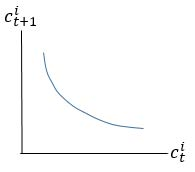
\includegraphics[width=0.3\textwidth]{Figures/intertemp_c_icurve.JPG}
\end{figure}
\end{frame}

%------------------------------------------------
%------------------------------------------------

\begin{frame}{Method \#2:\ Graphical}
Expand budget constraint
\begin{equation*}
a_{t+2}^{i}=R_{t+1}\left( R_{t}a_{t}^{i}+y_{t}^{i}-c_{t}^{i}\right)+y_{t+1}^{i}-c_{t+1}^{i}
\end{equation*}

Total differentiation taking $a_{t}^{i},a_{t+2}^{i},y_{t}^{i}$ and $y_{t+1}^{i}$ as given 
\begin{equation*}
\frac{dc_{t+1}^{i}}{dc_{t}^{i}}=-R_{t+1}=\text{MRT}
\end{equation*}

Budget constraint in $(c_{t}^{i},c_{t+1}^{i})$ space
\begin{figure}
\centering
\label{fig:intertemp_c_bconstraint}
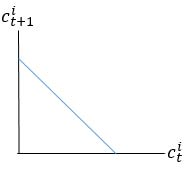
\includegraphics[width=0.3\textwidth]{Figures/intertemp_c_bconstraint.JPG}
\end{figure}
\end{frame}

%------------------------------------------------
%------------------------------------------------

\begin{frame}{Method \#2:\ Graphical}
Optimising household sets MRS=MRT 
\begin{equation*}
\beta R_{t+1}\frac{U_{c^{i},t+1}}{U_{c^{i},t}}-1=0
\end{equation*}
Optimality in $(c_{t}^{i},c_{t+1}^{i})$ space
\begin{figure}
\centering
\label{fig:intertemp_c_tangency}
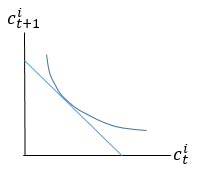
\includegraphics[width=0.3\textwidth]{Figures/intertemp_c_tangency.JPG}
\end{figure}
\end{frame}

%------------------------------------------------
%------------------------------------------------

\begin{frame}{Method \#3:\ Value function}
Value function (this is a very brief illustration of this advanced technique)
\begin{equation*}
V(a_{t}^{i})=\underset{a_{t+1}^{i}}{\max }\left[U(R_{t}a_{t}^{i}+y_{t}^{i}-a_{t+1}^{i})+\beta V(a_{t+1}^{i})\right]
\end{equation*}
First order condition still involves $V$, which is not yet explicitly, defined
\begin{equation*}
U_{c^{i},t}=\beta V^{\prime }(a_{t+1}^{i})
\end{equation*}
Differentiate $V(a_{t}^{i})$ w.r.t. $a_{t}^{i}$ (an \href{https://en.wikipedia.org/wiki/Envelope_theorem}{envelope condition} is being used) here)
\begin{equation*}
V^{\prime }(a_{t}^{i})=U_{c^{i},t}R_{t}
\end{equation*}
Then just roll forward one period and substitute for $V^{\prime }(a_{t+1}^{i})$
\begin{equation*}
\beta R_{t+1}\frac{U_{c^{i},t+1}}{U_{c^{i},t}}-1=0
\end{equation*}
\end{frame}

%------------------------------------------------
%------------------------------------------------

\begin{frame}{Method \#3:\ Value function}

Define (present value) Lagrangian
\begin{equation*}
\mathcal{L}^{i}=\underset{s=0}{\overset{\infty }{\sum }}\beta^{s}U(c_{t+s}^{i})+\underset{s=0}{\overset{\infty }{\sum }}\lambda_{t+s}^{i}\beta ^{s}\left(R_{t+s}a_{t+s}^{i}+y_{t+s}^{i}-c_{t+s}^{i}-a_{t+s+1}^{i}\right)
\end{equation*}

First order conditions 
\begin{equation*}
\begin{tabular}{llc}
$c_{t}^{i}$ & : & $U_{c^{i},t}=\lambda _{t}^{i}$ \\ 
$c_{t+1}^{i}$ & : & $U_{c^{i},t+1}=\lambda _{t+1}^{i}$ \\ 
$a_{t+1}^{i}$ & : & $\lambda_{t+1}^{i}\beta R_{t+1}-\lambda_{t}^{i}=0$
\end{tabular}
\end{equation*}

Combine to obtain the now familiar\ldots
\begin{equation*}
\beta R_{t+1}\frac{U_{c^{i},t+1}}{U_{c^{i},t}}-1=0
\end{equation*}
\end{frame}

%------------------------------------------------
%------------------------------------------------

\begin{frame}{Quick check\ldots}

Q: Does the following condition pin down the sequence of consumption that solves the household's problem?
\begin{equation*}
\beta R_{t+1}\frac{U_{c^{i},t+1}}{U_{c^{i},t}}-1=0
\end{equation*}

A: No, remember we need to satisfy the budget constraint
\begin{equation*}
\frac{a_{T+1}^{i}}{\tilde{R}_{T}}=a_{0}^{i}+\sum\limits_{t=0}^{T}\frac{y_{t}^{i}-c_{t}^{i}}{\tilde{R}_{t}}
\end{equation*}

The `Euler equation' shows how the slopes of the $U_{c,t}$ profile relate to the prevailing interest rate
	\begin{itemize}
	\item	Many ${c_{t}}_{t=0}^{\infty}$ sequences have the same slope, but are higher or lower
	\item	Only one will exhaust the household's resources exactly
	\end{itemize}
	
\end{frame}

%------------------------------------------------
%------------------------------------------------

\begin{frame}{Interpretation of Euler equation for consumption}

\begin{equation*}
\beta R_{t+1}\frac{U_{c^{i},t+1}}{U_{c^{i},t}}-1=0
\end{equation*}
Consider marginally less $c_{t}$
\begin{itemize}
\item	Cost: Foregoing utility from marginal unit of $c_{t}$
\item	Benefit: Extra saving $\Rightarrow$ utility $\uparrow$ from $c_{t+1}$ (traded at market rate, $R$)
\item	Marginal cost and marginal benefit should be equal at optimum
\end{itemize}

\vspace{3mm}
Re-arrange to see even more clearly
\begin{equation*}
\underbrace{\beta U_{c^{i},t+1} \times R_{t+1}}_{MB}=\underbrace{U_{c^{i},t}}_{MC}
\end{equation*}

\end{frame}

%------------------------------------------------
%------------------------------------------------

\begin{frame}{Interpretation of Euler equation for consumption}

\begin{equation*}
\beta R_{t+1}\frac{U_{c^{i},t+1}}{U_{c^{i},t}}-1=0
\end{equation*}

\textit{From the perspective of the price taking household}\ldots
\begin{itemize}
\item 	Growth in $U_{c^{i},t}$ is determined by $R_{t}$
\item	Change $R_{t}$ and the household will re-optimize
\item	Given a functional form for $U(\cdot)$ we can recover growth in $c_{t}$
\end{itemize}

\vspace{3mm}
Consider the following cases:
\begin{itemize}
\item $\beta R_{t+1}=1\rightarrow $ $U_{c^{i},t+1}=U_{c^{i},t}$ $\rightarrow$ $c_{t+1}^{i}=c_{t}^{i}$
\item $\beta R_{t+1}>1\rightarrow $ $U_{c^{i},t+1}<U_{c^{i},t}\rightarrow $ $c_{t+1}^{i}>c_{t}^{i}$
\item $\beta R_{t+1}<1\rightarrow $ $U_{c^{i},t+1}>U_{c^{i},t}\rightarrow $ $c_{t+1}^{i}<c_{t}^{i}$
\end{itemize}

\end{frame}

%------------------------------------------------
%------------------------------------------------

\begin{frame}{Interpretation of Euler equation for consumption}

\begin{equation*}
\beta R_{t+1}\frac{U_{c^{i},t+1}}{U_{c^{i},t}}-1=0
\end{equation*}

\textcolor{red}{\textit{From the perspective of the price taking household}\ldots}
\begin{itemize}
\item 	Growth in $U_{c^{i},t}$ is determined by $R_{t}$
\item	Change $R_{t}$ and the household will re-optimize
\item	Given a functional form for $U(\cdot)$ we can recover \textit{growth in} $c_{t}$
\end{itemize}

\vspace{3mm}
Consider the following cases:
\begin{itemize}
\item $\beta R_{t+1}=1\rightarrow $ $U_{c^{i},t+1}=U_{c^{i},t}$ $\rightarrow$ $c_{t+1}^{i}=c_{t}^{i}$
\item $\beta R_{t+1}>1\rightarrow $ $U_{c^{i},t+1}<U_{c^{i},t}\rightarrow $ $c_{t+1}^{i}>c_{t}^{i}$
\item $\beta R_{t+1}<1\rightarrow $ $U_{c^{i},t+1}>U_{c^{i},t}\rightarrow $ $c_{t+1}^{i}<c_{t}^{i}$
\end{itemize}

\end{frame}

%------------------------------------------------
%------------------------------------------------

\begin{frame}{General equilibrium}

So far, we haven't really made explicit the other parts of the economy
\begin{itemize}
\item	Suppose this is an endowment economy
\item	No firms
\item	No labor market
\item	No \textit{aggregate} saving technology (e.g. CA, government or capital)
\end{itemize}

Additionally, assume the households all have `log' utility
\[
U(c_{t}^{i}) = \log{(c_{t}^{i}}
\]
\end{frame}

%------------------------------------------------
%------------------------------------------------

\begin{frame}{General equilibrium}

Aggregate household Euler equations \emph{with log utility}
	\begin{itemize}
	\item	Add up both sides of household ($i$) Euler equations
	\end{itemize}
\begin{equation*}
\sum_{i}c_{t+1}^{i}=\beta R_{t+1}\sum_{i}c_{t}^{i}
\end{equation*}

Market clearing with no aggregate savings
\begin{itemize}
\item	\textbf{Equilibrium} $\Rightarrow$ agents' atomistic decisions are consistent in aggregate
\end{itemize}
\begin{equation*}
\sum_{i}y_{t}^{i}=\sum_{i}c_{t}^{i}\ \ \text{for }\forall t
\end{equation*}

Market interest rate
\begin{itemize}
\item	Solve for (endogenous) $R_{t}$
\item	H'holds don't care about market clearing, they optimize given prices
\item	\textbf{Prices must be such that the aggregate endowment is equal to aggregate consumption}
\end{itemize}
\begin{equation*}
\beta R_{t+1}=\frac{\sum_{i}y_{t+1}^{i}}{\sum_{i}y_{t}^{i}}
\end{equation*}

\end{frame}

%------------------------------------------------
%------------------------------------------------

\begin{frame}{General equilibrium - Representative agent}

Let us define `aggregate' consumption:
\[
c_{t} \equiv \sum\limits_{i} c_{t}^{i}
\]
and `aggregate' output $y_{t}$
\[
y_{t} \equiv \sum\limits_{i} y_{t}^{i}
\]

Clearly, by our previous discussion, $c_{t}=y_{t}$

\end{frame}

%------------------------------------------------
%------------------------------------------------

\begin{frame}{General equilibrium - Representative agent}

Aggregate household Euler equations \emph{with log utility}
	\begin{itemize}
	\item	Add up both sides of household ($i$) Euler equations
	\end{itemize}
\begin{equation*}
\sum_{i}c_{t+1}^{i}=\beta R_{t+1}\sum_{i}c_{t}^{i}
\end{equation*}

Market clearing with no aggregate savings
\begin{itemize}
\item	\textbf{Equilibrium} $\Rightarrow$ agents' atomistic decisions are consistent in aggregate
\end{itemize}
\begin{equation*}
\sum_{i}y_{t}^{i}=\sum_{i}c_{t}^{i}\ \ \text{for }\forall t
\end{equation*}

Market interest rate
\begin{itemize}
\item	Solve for (endogenous) $R_{t}$
\item	H'holds don't care about market clearing, they optimize given prices
\item	\textbf{Prices must be such that the aggregate endowment is equal to aggregate consumption}
\end{itemize}
\begin{equation*}
\beta R_{t+1}=\frac{\sum_{i}y_{t+1}^{i}}{\sum_{i}y_{t}^{i}}
\end{equation*}

\end{frame}

%------------------------------------------------
%------------------------------------------------

\begin{frame}{General equilibrium - Representative agent}

Aggregate household Euler equations \emph{with log utility}
	\begin{itemize}
	\item	Add up both sides of household ($i$) Euler equations
	\end{itemize}
\begin{equation*}
\sum_{i}c_{t+1}^{i}=\beta R_{t+1}\sum_{i}c_{t}^{i}
\end{equation*}

Market clearing with no aggregate savings
\begin{itemize}
\item	\textbf{Equilibrium} $\Rightarrow$ agents' atomistic decisions are consistent in aggregate
\end{itemize}
\begin{equation*}
\sum_{i}y_{t}^{i}=\sum_{i}c_{t}^{i}\ \ \text{for }\forall t
\end{equation*}

Market interest rate
\begin{itemize}
\item	Solve for (endogenous) $R_{t}$
\item	H'holds don't care about market clearing, they optimize given prices
\item	\textbf{Prices must be such that the aggregate endowment is equal to aggregate consumption}
\end{itemize}
\begin{equation*}
\beta R_{t+1}=\frac{\sum_{i}y_{t+1}^{i}}{\sum_{i}y_{t}^{i}}
\end{equation*}

\end{frame}

%------------------------------------------------
%------------------------------------------------

\begin{frame}{General equilibrium - Representative agent}

Aggregate household Euler equations \emph{with log utility}
	\begin{itemize}
	\item	Add up both sides of household ($i$) Euler equations
	\end{itemize}
\begin{equation*}
\textcolor{red}{c_{t+1}=\beta R_{t+1}\sum_{i}c_{t}}
\end{equation*}

Market clearing with no aggregate savings
\begin{itemize}
\item	\textbf{Equilibrium} $\Rightarrow$ agents' atomistic decisions are consistent in aggregate
\end{itemize}
\begin{equation*}
\textcolor{red}{y_{t}=c_{t}\ \ \text{for }\forall t}
\end{equation*}

Market interest rate
\begin{itemize}
\item	Solve for (endogenous) $R_{t}$
\item	H'holds don't care about market clearing, they optimize given prices
\item	\textbf{Prices must be such that the aggregate endowment is equal to aggregate consumption}
\end{itemize}
\begin{equation*}
\textcolor{red}{\beta R_{t+1}=\frac{y_{t+1}}{y_{t}}}
\end{equation*}

\end{frame}

%------------------------------------------------
%------------------------------------------------

\begin{frame}{General equilibrium - Representative agent}

The same conditions we had before are satisfied under the aggregate (and under the `average' - divide by $N$ or integrate over a mass of households)
\begin{itemize}
\item	This shows that this economy admits a `representative' agent
\item	Equilibrium prices and aggregate/average quantities can be obtained as if there were one `representative' (competitive) household with the aggregate endowment process as its `income'
\end{itemize}

\vspace{2mm}
Note, we haven't said all households have the same $c_{i,t}$ or $y_{i,t}$
\begin{itemize}
\item	Doesn't matter for aggregates or solving for $R_{t}$ in this case
\item	To obtain them, simply use $R_{t}$, Euler equation and budget constraint and whatever $y_{t}^{i}$ is relevant to your problem/case
\item	Any split of the $y_{t}$ pie into individual $y^{i}_{t}$ will be consistent with the aggregate endogenous variables found
\end{itemize}

\vspace{2mm}
Note, also, the importance that they were facing the same prices

\end{frame}

%------------------------------------------------
%------------------------------------------------

\begin{frame}{General equilibrium - Some subtle points}

Recall the condition
\begin{equation*}
\beta R_{t+1}=\frac{y_{t+1}}{y_{t}}
\end{equation*}
and compare with the Euler equation of a given household, $i$
\begin{equation*}
\beta R_{t+1}=\frac{c^{i}_{t+1}}{c^{i}_{t}}
\end{equation*}

In the latter case, we could talk about the interest rate \textit{causing} consumption growth for the household
\begin{itemize}
\item	The household is a price taker and does not individually affect $R$
\end{itemize}

\vspace{2mm}
In the former, our equilibrium assumption $\Rightarrow$ the \textit{exogenously specified} $y_{t}$ process necessitates a particular $R_{t}$
\begin{itemize}
\item	In richer models (with labor, capital accumulation etc.) `output growth' will also be endogenous
\item	Causal relations between endogenous variables are tricky in an equilibrium and may involve feedback
\end{itemize}
\end{frame}


\section{Ramsey Growth Model}

\begin{frame}

\begin{center}
{\LARGE Ramsey Growth Model}
\end{center}

\end{frame}

%------------------------------------------------
%------------------------------------------------

\begin{frame}{Ramsey model}

Production economy, rather than endowment
\begin{itemize}
\item Log utility
\item Labor supply exogenous (constant and normalized to unity)
\item Constant returns to scale in production function
\item $100\%$ depreciation of capital (`investment' in $t$ = $K_{t+1}$)
\item Technology, $\theta_{t}$, grows at rate $g$
\item Infinitely-lived \textit{representative} agent
\end{itemize}

\end{frame}

%------------------------------------------------
%------------------------------------------------

\begin{frame}{Household problem in Ramsey}

Representative household maximizes lifetime utility
\begin{gather*}
\underset{\{C_{t+s},K_{t+s+1}\}}{\max }\underset{s=0}{\overset{\infty }{\sum}}\beta ^{s}\log C_{t+s} \\
\text{s.t.} \\
K_{t+s+1}=r_{t+s}K_{t+s}+w_{t+s}- C_{t+s} \; \forall s\geq 0 \\
K_{t}\text{ given,} \\
\underset{T\rightarrow \infty }{\lim }\frac{K_{T+1}}{\tilde{R}_{T}}\geq 0
\end{gather*}

Euler equation for consumption as before
\begin{equation*}
\frac{C_{t+1}}{\beta C_{t}}=r_{t+1}
\end{equation*}

\end{frame}

%------------------------------------------------
%------------------------------------------------

\begin{frame}{Household problem in Ramsey}

Representative household maximizes lifetime utility
\begin{gather*}
\underset{\{C_{t+s},K_{t+s+1}\}}{\max }\underset{s=0}{\overset{\infty }{\sum}}\beta ^{s}\log C_{t+s} \\
\text{s.t.} \\
\overbrace{K_{t+s+1}}^{Investment}=\overbrace{\underbrace{r_{t+s}K_{t+s}+w_{t+s}}_{Earnings}- C_{t+s}}^{Savings} \; \forall s\geq 0 \\
K_{t}\text{ given,} \\
\underset{T\rightarrow \infty }{\lim }\frac{K_{T+1}}{\tilde{R}_{T}}\geq 0
\end{gather*}

Euler equation for consumption as before
\begin{equation*}
\frac{C_{t+1}}{\beta C_{t}}=r_{t+1}
\end{equation*}

\end{frame}

%------------------------------------------------
%------------------------------------------------

\begin{frame}{Household problem in Ramsey}

Representative household maximizes lifetime utility
\begin{gather*}
\underset{\{C_{t+s},K_{t+s+1}\}}{\max }\underset{s=0}{\overset{\infty }{\sum}}\beta ^{s}\log C_{t+s} \\
\text{s.t.} \\
K_{t+s+1}=r_{t+s}K_{t+s}+w_{t+s} \textcolor{red}{\underbrace{L_{t}^{S}}_{\equiv 1}}- C_{t+s} \; \forall s\geq 0 \\
K_{t}\text{ given,} \\
\underset{T\rightarrow \infty }{\lim }\frac{K_{T+1}}{\tilde{R}_{T}}\geq 0
\end{gather*}

Euler equation for consumption as before
\begin{equation*}
\frac{C_{t+1}}{\beta C_{t}}=r_{t+1}
\end{equation*}

\end{frame}

%------------------------------------------------
%------------------------------------------------

\begin{frame}{Firm problem in Ramsey}

Firm maximizes profits
\begin{equation*}
\underset{K_{t},L^{D}_{t}}{\max }\left( K_{t}^{\alpha }\left( \theta_{t}L^{D}_{t}\right) ^{1-\alpha }-w_{t}L^{D}_{t}-r_{t}K_{t}\right)
\end{equation*}

First order conditions define factor prices as before
\begin{eqnarray*}
r_{t} &=&\alpha K_{t}^{\alpha -1}\left( \theta _{t}L^{D}_{t}\right) ^{1-\alpha }\\
w_{t} &=&\left( 1-\alpha \right) K_{t}^{\alpha }\theta _{t}\left( \theta_{t}L^{D}_{t}\right) ^{-\alpha }
\end{eqnarray*}

\end{frame}

%------------------------------------------------
%------------------------------------------------

\begin{frame}{Firm problem in Ramsey}

Why have I written $L_{t}^{D}$ and $L_{t}^{S}$ rather than $L_{t}$?
\begin{itemize}
\item	$L_{t}^{S}\equiv 1$ isn't important
\item	What \textit{is} important is that outside equilibrium (without appropriate `prices') there's no reason to think $L_{t}^{S}=L_{t}^{D}$
\item	We need $w_{t}$ and $r_{t}$ to (among other things) induce firms to set $L_{t}^{D}$ - thus clearing markets
\end{itemize}

\vspace{1.5mm}
$L_{t}^{S}=L_{t}^{D}$ is an equilibrium condition
\begin{itemize}
\item	Incorporating it allows us to use $L_{t}$ as the amount of labor (supplied and demanded) in equilibrium
\item	I should really be doing this for $K_{t}^{S}$ and $K_{t}^{D}$ but life's too short and typos too numerous\ldots
\end{itemize}

\vspace{1.5mm}
In a price taking world, who sets the prices to the `necessary' values?
\begin{itemize}
\item	Hmmmm,\ldots ponder\ldots
\item	Anyway, regardless, these prices induce an equilibrium
\end{itemize}

\end{frame}

%------------------------------------------------
%------------------------------------------------

\begin{frame}{Equilibrium in Ramsey}

A competitive equilibrium is a sequence 
\begin{equation*}
\left\{ r_{t},w_{t},C_{t},K_{t},L_{t}\right\} _{t=0}^{\infty }
\end{equation*}

s.t.

\begin{enumerate}
\item $\left\{ C_{t},K_{t+1}\right\} $ solves household problem given $\left\{ r_{t},w_{t}\right\} $
\item $\left\{ K_{t},L_{t}\right\} $ solves firm problem given $\left\{r_{t},w_{t}\right\} $
\item Markets clear $L_{t}=1$ and $C_{t}+K_{t+1}=Y_{t}=K_{t}^{\alpha }\left(\theta _{t}L_{t}\right) ^{1-\alpha }$
\item $K_{t}$ given
\item TVC
\end{enumerate}

\end{frame}

%------------------------------------------------
%------------------------------------------------

\begin{frame}{Equilibrium in Ramsey}

Euler equation for consumption and return to capital imply
\begin{equation*}
\frac{1}{C_{t}}=\alpha \beta \frac{1}{C_{t+1}}K_{t+1}^{\alpha -1}\left(\theta _{t+1}L_{t+1}\right) ^{1-\alpha }
\end{equation*}

Substitute in for market clearing conditions and rearrange
\begin{equation*}
\frac{Y_{t+1}}{C_{t+1}}=-\frac{1}{\alpha \beta }+\frac{1}{\alpha \beta } \frac{Y_{t}}{C_{t}}
\end{equation*}

\vspace{2mm}
Only stable solution is $\frac{Y_{t}}{C_{t}} = \frac{1}{1-\alpha \beta} \; \forall t\geq 0$

\end{frame}

%------------------------------------------------
%------------------------------------------------

\begin{frame}{Equilibrium in Ramsey}

\begin{figure}
\centering
\label{fig:ramsey_transversality}
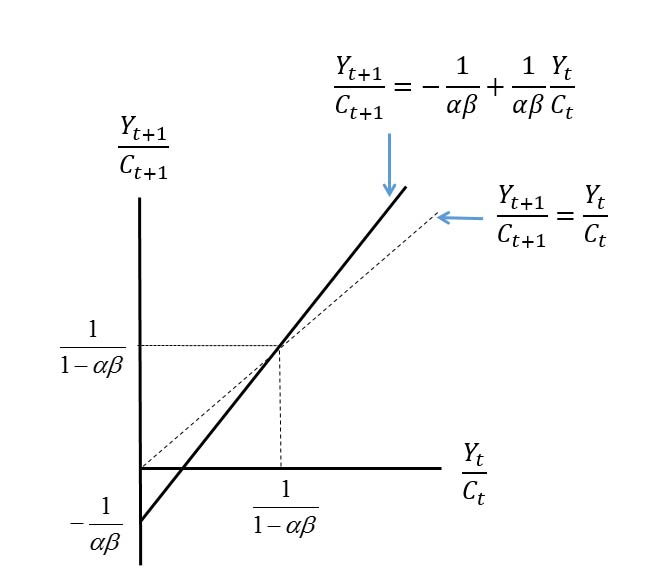
\includegraphics[width=0.6\textwidth]{Figures/ramsey_transversality.JPG}
\end{figure}

Only stable solution is $\frac{Y_{t}}{C_{t}} = \frac{1}{1-\alpha \beta} \; \forall t\geq 0$

\end{frame}

%------------------------------------------------
%------------------------------------------------

\begin{frame}{Equilibrium in Ramsey with technological change}

\begin{itemize}
\item $Y_{t}/C_{t},$ $Y_{t}/K_{t+1}$ constant
\item $\theta _{t},C_{t},K_{t},Y_{t}$ grow at rate $g$
\item $r_{t}=\alpha K_{t}^{\alpha -1}\left( \theta _{t}L_{t}\right)^{1-\alpha }$ $=\alpha \tilde{K}_{t}^{\alpha -1}$ constant
\item $w_{t}=\left( 1-\alpha \right) K_{t}^{\alpha }\theta _{t}\left( \theta_{t}L_{t}\right) ^{-\alpha }=\left( 1-\alpha \right) \theta _{t}\tilde{K}_{t}^{\alpha }$ grows at rate $g$
\end{itemize}

\end{frame}

%------------------------------------------------
%------------------------------------------------

\begin{frame}{Check Kaldor (1957) facts}

\begin{enumerate}
\item Output per worker grows at a roughly constant rate \textcolor{red}{YUP}
\item Capital per worker grows over time \textcolor{red}{YUP}
\item Capital/output ratio is roughly constant \textcolor{red}{YUP}
\item Rate of return to capital is constant \textcolor{red}{YUP}
\item Shares of capital and labor in net income are nearly constant \textcolor{red}{YUP}
\item Real wage grows over time \textcolor{red}{YUP}
\item Ratios of consumption and investment to GDP\ are constant \textcolor{red}{YUP}
\end{enumerate}

\end{frame}

%------------------------------------------------
%------------------------------------------------

\begin{frame}{Endogenous growth models}

Growth is exogenous in this model
	\begin{itemize}
	\item	$\theta_{t}$ an exogenous process
	\end{itemize}
\vspace{2mm}
\textit{Endogenous} growth models seek to explain growth
	\begin{itemize}
	\item	Not covering in depth - but may be in a problem set, say
	\end{itemize}
\vspace{2mm}
\textbf{Extended accumulation} \textbf{models}
	\begin{itemize}
	\item	Overcome diminishing returns to capital by adding externalities in capital accumulation (learning-by-doing and AK model)
	\item	Alternatively, additional factors of production (human capital)
	\end{itemize}
\vspace{2mm}
\textbf{Innovation models}
	\begin{itemize}
	\item	Explain technological progress as a function of endogenous variables
	\item	E.g. Investment in R\&D
	\end{itemize}

\end{frame}

%------------------------------------------------
%------------------------------------------------

\begin{frame}{Growth accounting}

Take logs (see lect. 1) and differentiate $Y_{t}=K_{t}^{\alpha }\left( \theta_{t}L_{t}\right) ^{1-\alpha }$ to decompose into weighted percentage growth rates
\begin{equation*}
\frac{1}{Y_{t}}\frac{dY_{t}}{dt}=\alpha \frac{1}{K_{t}}\frac{dK_{t}}{dt}+(1-\alpha )\frac{1}{\theta_{t}}\frac{d\theta_{t}}{dt}+(1-\alpha )\frac{1}{L_{t}}\frac{dL_{t}}{dt}
\end{equation*}

\vspace{5mm}
Capital share of income in equilibrium$=\alpha$, so set $\approx 1/3$ (as in historical data)
\begin{eqnarray*}
\text{Growth in }Y_{t}\text{ } &=&\frac{1}{3}\times \text{Growth in }K_{t} \\
&&+\frac{2}{3}\times \left( \text{Growth in }\theta _{t}+\text{Growth in }L_{t}\right)
\end{eqnarray*}

\end{frame}

%%------------------------------------------------
%%------------------------------------------------

\begin{frame}{Growth accounting in the $20^{th}$ century, Crafts (2000)}

\begin{figure}
\centering
\subfigure{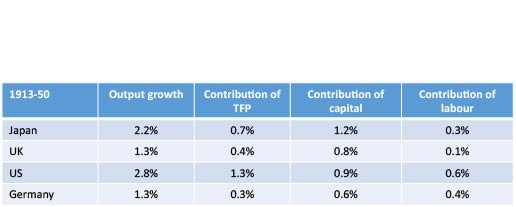
\includegraphics[width=0.45\textwidth]{Figures/growth_1913_50.JPG}}\\
\subfigure{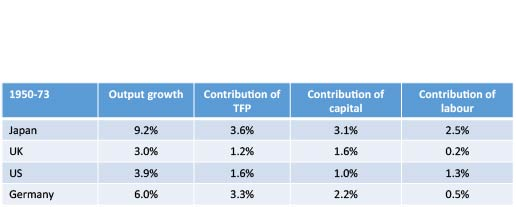
\includegraphics[width=0.45\textwidth]{Figures/growth_1950_73.JPG}}\\
\subfigure{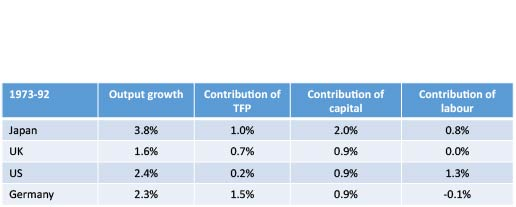
\includegraphics[width=0.45\textwidth]{Figures/growth_1970_92.JPG}}
\end{figure}

\end{frame}

%------------------------------------------------
%------------------------------------------------

\begin{frame}{Growth accounting in emerging markets 1960-1994}
\begin{figure}
\centering
\label{fig:growth_decomp}
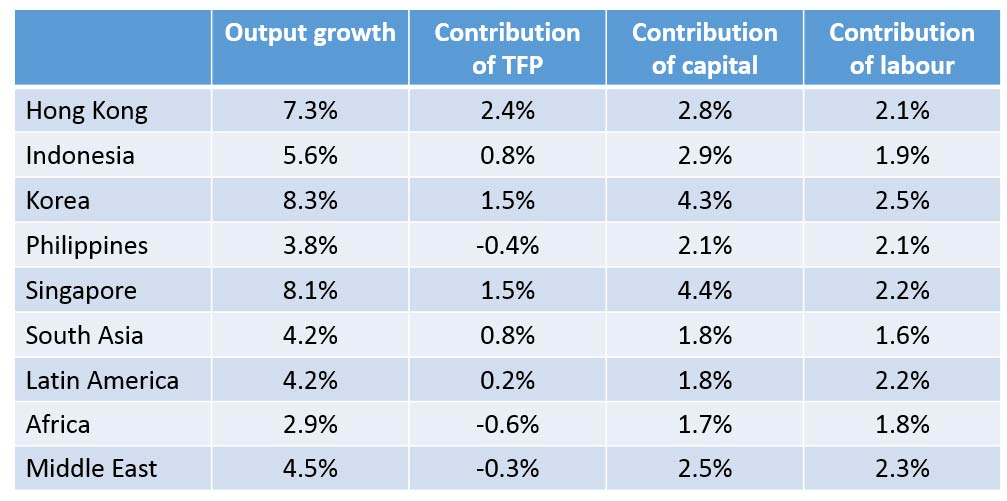
\includegraphics[width=0.8\textwidth]{Figures/growth_decomp.JPG}
\end{figure}
\end{frame}

%------------------------------------------------
%------------------------------------------------

\begin{frame}{Growth accounting for the UK 1970-2013, ONS\ (2015)}

\begin{figure}
\centering
\label{fig:growth_decomp}
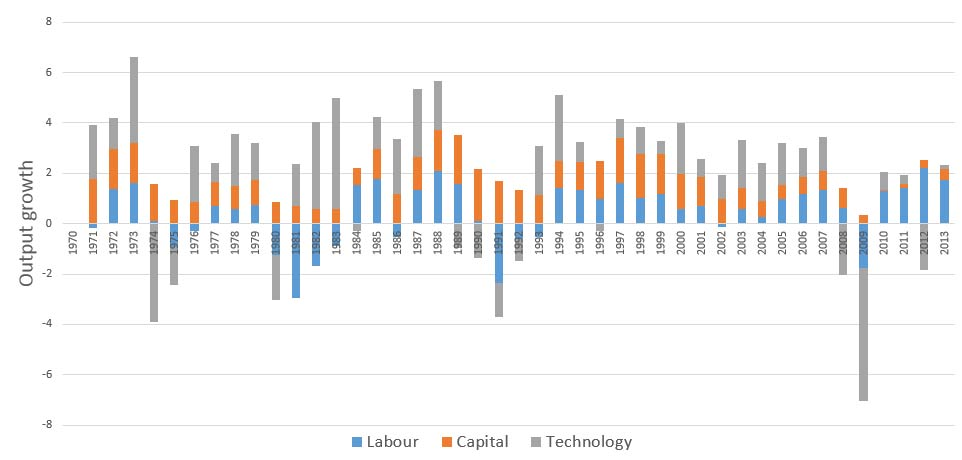
\includegraphics[width=0.8\textwidth]{Figures/growth_decomp_chart.JPG}
\end{figure}

Average UK growth of $2.1\%$
	\begin{itemize}
	\item	$0.4\%$ from technology
	\item	$0.2\%$ from capital
	\item	$0.5\%$ from labor
	\end{itemize}

\end{frame}

\section{Monetary Models - Background}

\begin{frame}

\begin{center}
{\LARGE Monetary Models - Background}
\end{center}

\end{frame}

%-------------------------------------------------------
\subsection{History Lesson}
%-------------------------------------------------------

\begin{frame}{Quantity theory of money}

Much discussion (though not in recent years) of the effects of monetary policy began with some form of the following equation
\begin{equation}
M_{t}V_{t} \equiv P_{t}Y_{t} \label{eqn:mvpy}
\end{equation}
where $M_{t}$ is the quantity of money, $V_{t}$ the velocity of its circulation, $P_{t}$ the general price level and $Y_{t}$ real output.

\vspace{2mm}
Equation (\ref{eqn:mvpy}) is an \emph{identity} (always true by definition)
\begin{itemize}
\item Holds regardless of CB targeting interest rate, $i_{t}$, or $M$ directly
\item Uninteresting unless a theory restricts behavior of at least one variable
\end{itemize}

\vspace{2mm}
(Long run) `classical dichotomy' / `quantity theory of money'
\begin{itemize}
\item In the long run, $Y$ and $V$ are determined by non-monetary factors
\item Thus, M and P move 1:1 in the long run
\end{itemize}

\end{frame}

%-------------------------------------------------------

%-------------------------------------------------------

\begin{frame}{Quantity theory of money}

Economists agree about little but\ldots
\begin{itemize}
\item 	The \emph{long run} classical dichotomy is arguably an exception
\item 	Long run growth determined by `supply' factors - not monetary
\item 	In LR, monetary factors only influence \emph{nominal}, but not \emph{real} variables
\item	Long run correlations between $M$ and $P$ $\approx 1$ in the data
\end{itemize}

\vspace{2mm}
Almost complete consensus that \emph{`there is no long-run trade-off between the rate of inflation and the rate of unemployment'} - Taylor (1996)
%\begin{itemize}
%\item	Caveat: Zero lower bound and the probability of monetary policy being constrained in low inflation environments
%\item	Caveat: High inflation may correlate with volatile inflation and mismanaged policy affecting economic activity
%\item	But the long run classical dichotomy is generally thought of as a given
%\end{itemize}

\end{frame}

%-------------------------------------------------------

%-------------------------------------------------------

\begin{frame}{Fisher equation}

Its rare nowadays for central banks to use $M_{t}$ as an explicit policy tool
\begin{itemize}
\item	Typically now set a short term nominal interest rate, $i_{t}$
\item	Given `money demand', the central bank adapts money supply so market clears at desired $i_{t}$
\end{itemize}

\vspace{2mm}
In this context, the `quantity equation' is less intuitive - instead the `Fisher equation' is useful to aid understanding
\begin{eqnarray}
i_{t} = r_{t} + E_{t}[ \pi_{t+1} ] 
\end{eqnarray}
where $i_{t}/r_{t}$ is the nominal/real interest rate and $\pi_{t}$ is (net) inflation.

\vspace{2mm}
The (long run) classical dichotomy implies that $r_{t}$ is unrelated to monetary factors
\begin{itemize}
\item	$i_{t}$ and inflation move 1:1, conditional on $r_{t}$
\item	If $r_{t}$ changes without a change in $i_{t}$ inflation adjusts
\end{itemize}

\end{frame}

%-------------------------------------------------------
\subsection{Effects of Monetary Policy}
%-------------------------------------------------------

\begin{frame}{Interaction of real and nominal factors}

In the shorter run the classical dichotomy is not broadly accepted
\begin{itemize}
\item 	Money/interest rates and output (or other measures of activity, such as unemployment) appear to co-move
\item	Central banks' activities are predicated on the assumption that changing $i_{t}$ induces a change in $r_{t}$
\end{itemize}

\vspace{2mm}
Co-movements are suggestive that there is a connection between real and nominal variables (see Ch. 1 Walsh)
\begin{itemize}
\item	Lead-lag correlations $\Rightarrow$ high $M_{t}$ typically precedes high $Y_{t}$
\item	Cyclical movements in money track those of GDP growth fairly well until early 80s
\item	Short term nominal rates generally track - and somewhat precede - cyclical movements in GDP
\end{itemize}
 
\end{frame}

%-------------------------------------------------------

%-------------------------------------------------------

\begin{frame}{Interaction of real and nominal factors}

\begin{figure}[!htb]
\center{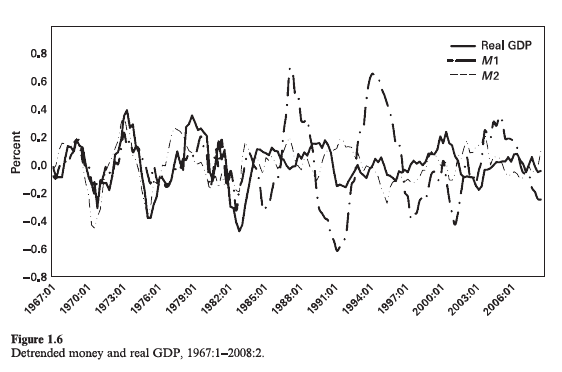
\includegraphics[width=0.8\textwidth]{Figures/detrend_M_and_GDP_walsh_ch1.png}}
\caption{\label{fig:walsh_ch1_M_GDP} De-trended money and output (from Walsh Ch.1)}
\end{figure}
 
\end{frame}

%-------------------------------------------------------

%-------------------------------------------------------

\begin{frame}{Interaction of real and nominal factors}

\begin{figure}[!htb]
\center{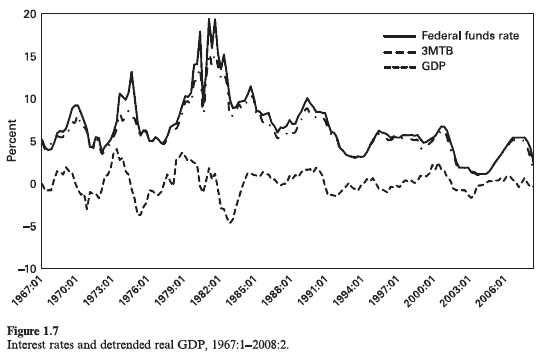
\includegraphics[width=0.8\textwidth]{Figures/i_rate_detrend_gdp_walsh_ch1.png}}
\caption{\label{fig:walsh_ch2_M_GDP} Short rate and de-trended output (from Walsh Ch.1)}
\end{figure}
 
\end{frame}

%-------------------------------------------------------

%-------------------------------------------------------

\begin{frame}{Interaction of real and nominal factors}

Difficult to disentangle direction of causality
\begin{itemize}
\item	Are these movements \emph{induced} by monetary policy or is policy \emph{responding} to the economy?
\item	Even if policy variable appears to lead activity, we face the \emph{post hoc ergo propter hoc} fallacy
\end{itemize}

\vspace{2mm}
Want to examine periods after an unanticipated `shock' from policymakers
\begin{itemize}
\item	Derives purely from policymaker - not economy - and thus closer to a `natural experiment'
\item	Then estimate propagation of shock through economy
	\begin{itemize}
	\item	If $M_{t}$ is the tool, does it affect $M/P$ and real activity, rather than passing 1:1 into prices? - Recall `quantity theory'
	\item	If $i_{t}$ is the tool, does it affect $r_{t}$ and real activity, rather than passing 1:1 into $E_{t}[\pi_{t+1}]$? - Recall Fisher equation
	\end{itemize}
%\item	May be possible to combine with a model to estimate `structural parameters' (more on this later\ldots)
\end{itemize}

\end{frame}

%-------------------------------------------------------

%-------------------------------------------------------

\begin{frame}{Identifying monetary policy shocks and their effects}

Friedman and Schwarz (1963) and narrative approaches
\begin{itemize}
\item Seminal work on influence of monetary policy in the U.S. (most notably in the Great Depression)
	\begin{itemize}
	\item	Documentary evidence to isolate $\Delta M$ unrelated to economic conditions
	\item	Suggests that fluctuations in money supply led to those in real activity
	\item	Related to case study analyses of disinflationary policy (Sargent (1986))
	\end{itemize}
\item Influential - but problematic elements in empirical approach
	\begin{itemize}
	\item 	Later support from Romer and Romer (1989) in a more modern form
	\item	Further strengthened by Romer and Romer (2004)
	\end{itemize}
\end{itemize}

\vspace{2mm}
Other recent work on obtaining measures of policy surprises
\begin{itemize}
\item	Nakamura and Steinsson (2013) and Gertler Karadi (2015) use `high frequency information'
\item	Look at asset price movements in short intervals around FOMC announcements to identify `surprises'
\end{itemize}

\end{frame}

%-------------------------------------------------------

%-------------------------------------------------------

\begin{frame}{Identifying monetary policy shocks and their effects}

\begin{quotation}
On three occasions the System deliberately took policy steps of major magnitude which cannot be regarded as necessary or inevitable economic consequences of contemporary changes in money income and prices. Like the crucial experiments of the physical scientist, the results are so consistent and sharp as to leave little doubt about their interpretation. The dates are January-June 1920, October 1931, and June 1936-January 1937
\end{quotation}
\center - Friedman and Schwarz, 1963, p.688

\end{frame}

%-------------------------------------------------------

%-------------------------------------------------------

\begin{frame}{Identifying monetary policy shocks and their effects}

\begin{quotation}
There was another major anti-inflationary shock to monetary policy on October 6, 1979. In effect, the Federal Reserve decided that its measures over the previous year had been unsuccessful in reducing inflation and that much stronger measures were needed. Although the shift in policy was to some extent presented as a technical change, the fact that it was intended to lead to considerably higher interest rates and lower money growth was clear. For example, "the Committee anticipated that the shift . . . would result in ... a prompt increase ... in the federal funds rate"
\end{quotation}
\center - Romer and Romer, 1989, p.142

\end{frame}

%-------------------------------------------------------

%-------------------------------------------------------

\begin{frame}{Identifying monetary policy shocks and their effects}

Friedman and Schwarz (1963) and narrative approaches
\begin{itemize}
\item Seminal work on influence of monetary policy in the U.S. (most notably in the Great Depression)
	\begin{itemize}
	\item	Documentary evidence to isolate $\Delta M$ unrelated to economic conditions
	\item	Suggests that fluctuations in money supply led to those in real activity
	\item	Related to case study analyses of disinflationary policy (Sargent (1986))
	\end{itemize}
\item Influential - but problematic elements in empirical approach
	\begin{itemize}
	\item 	Later support from Romer and Romer (1989) in a more modern form
	\item	Further strengthened by Romer and Romer (2004)
	\end{itemize}
\end{itemize}

\vspace{2mm}
Other recent work on obtaining measures of policy surprises
\begin{itemize}
\item	Nakamura and Steinsson (2013) and Gertler Karadi (2015) use `high frequency information'
\item	Look at asset price movements in short intervals around FOMC announcements to identify `surprises'
\end{itemize}

\end{frame}

%-------------------------------------------------------

%-------------------------------------------------------

\begin{frame}{Vector Autoregressions}

Another powerful approach to assessing the impact of monetary policy shocks is Vector Autoregression (VAR) analysis (see Walsh Ch. 1 for this example)

\vspace{3mm}
\begin{quotation}
While researchers have disagreed on the best means of identifying policy shocks, there has been a surprising consensus on the general nature of the economic responses to monetary policy shocks. A variety of VARs estimated for a number of countries all indicate that, in response to a policy shocks, output follows a hump-shaped pattern in which the peak impact occurs several quarters after the initial shock.
\end{quotation}
\begin{center}
- Walsh, 1998, p.31
\end{center}

\vspace{3mm}
See discussion in lecture 1

\end{frame}

%-------------------------------------------------------

%-------------------------------------------------------

\begin{frame}{Vector Autoregressions}

\begin{figure}[!htb]
\center{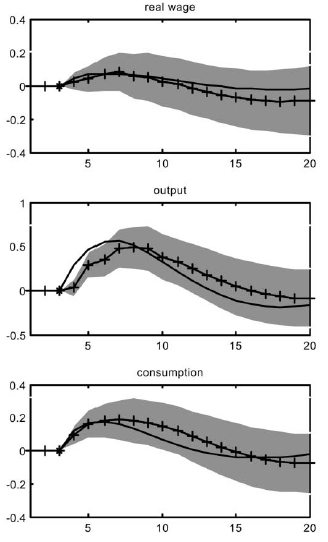
\includegraphics[width=0.30\textwidth]{Figures/cee2005_fig1_subset2}}
\caption{\label{fig:cee05_2} Subset of IRFs from CEE (2005)}
\end{figure}

\end{frame}

%-------------------------------------------------------

%-------------------------------------------------------

\begin{frame}{Vector Autoregressions}

\begin{figure}[!htb]
\center{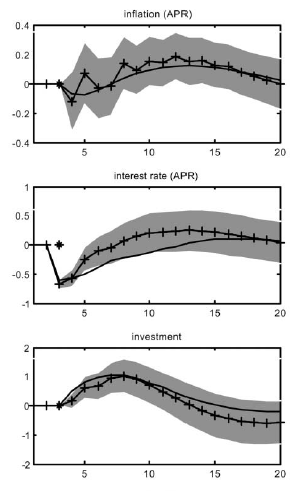
\includegraphics[width=0.30\textwidth]{Figures/cee2005_fig1_subset1}}
\caption{\label{fig:cee05_1} Subset of IRFs from CEE (2005)}
\end{figure}

\end{frame}

%-------------------------------------------------------

%-------------------------------------------------------

\begin{frame}{Vector Autoregressions}

VAR approach useful but not without flaws/critics\ldots
\vspace{2mm}
\begin{itemize}
\item 	Monetary policy shocks are now likely rare/small (Ramey (2016))
	\begin{itemize}
	\item	Makes it more difficult to use \emph{policy} shocks to estimate impact of policy
	\item	Can still estimate role of policy but need \emph{other} shocks \textbf{and} a model
	\end{itemize}
\vspace{1mm}
\item	Changes in underlying parameters (Lucas critique and Rational Expectations)
	\begin{itemize}
	\item	Response to shocks depends on parameters describing policymakers' approach \textbf{and} all other parameters in the economy (e.g. regulation, preferences\ldots)
	\item	If they change, previous estimates may become obsolete
	\end{itemize}
\vspace{1mm}	
\item 	Responses may not be accurately recovered even from data generated by a model (Chari \emph{et al} (2008))
	\begin{itemize}
	\item	Can still use, but in a `moment matching' exercise \emph{involving a model}
	\item	VARs on actual data and on data from model - minimize discrepancy
	\end{itemize}
\end{itemize}

\end{frame}

%-------------------------------------------------------

%-------------------------------------------------------

\begin{frame}{Vector Autoregressions}

More problems with VAR analysis\ldots
\vspace{2mm}
\begin{itemize}
\item	Unhelpful for welfare analysis
	\begin{itemize}
	\item	Knowing that policy affects activity is one thing\ldots
	\item 	\ldots but knowing \emph{how it should try to affect it} is another
	\item 	Agent's optimization problems must be explicit for micro-founded welfare analysis
	\item 	VARs are silent on this
	\end{itemize}
\item	Story telling / incorporation of microeconomic evidence
	\begin{itemize}
	\item 	Policymakers like to understand/explain transmission mechanism
	\item	Elements of models (such as, say, household risk aversion) can be pinned down by evidence from experiments/more granular research
	\item	Not possible with VARs (or very difficult)
	\end{itemize}
\end{itemize}

\vspace{2mm}
A lot of these `problems' can be addressed by using a model\ldots

\end{frame}

%-------------------------------------------------------
\subsection{DSGE Models}
%-------------------------------------------------------

\begin{frame}{Role of monetary policy - DSGE models}

DSGE models initially associated with the `Real Business Cycle' literature
\begin{itemize}
\item	Seminal work of Kydland and Prescott (1982) and Prescott (1986)
\item	No (or minor) distortions $\Rightarrow$ despite fluctuations (the `business cycle') the economy is always efficient
\item	Limited role of monetary policy - main shocks were `real' (technology)
\end{itemize}

\vspace{2mm}
Beautiful models - but unsatisfactory in various dimensions
\begin{itemize}
\item	If monetary policy was included, optimal policy looked nothing like real world practice
\item	Effects of policy shocks often counterfactual (recall evidence discussed above)
\item	Hard to reconcile dominant role of technology shocks with\ldots
	\begin{itemize}
	\item	\emph{Unconditional} positive comovement of employment and output in data
	\item	Empirical studies $\Rightarrow$ \emph{technology} shocks move them in opposite direction
	\end{itemize}
\end{itemize}

\end{frame}

%-------------------------------------------------------

%-------------------------------------------------------

\begin{frame}{Role of monetary policy - DSGE models}

The challenge:
\begin{itemize}
\item	Keep the `good' aspects of RBC models\ldots
\item	\ldots while enhancing ability to explain and justify monetary policy
\end{itemize}

\end{frame}

%-------------------------------------------------------

%-------------------------------------------------------

\begin{frame}{Role of monetary policy - DSGE models}

New Keynesian modeling was a response to this challenge
\vspace{2mm}
\begin{itemize}
\item	Interpret as a \textbf{micro-founded} formalization of `Keynesian' ideas
	\begin{itemize}
	\item	IS-LM analysis `much less careful' - rather \emph{ad hoc}
	\item	`We are an equation short' (Keynes) - price setting not modeled
	\end{itemize}
\vspace{1mm}
\item	Emphasis on \textbf{nominal rigidities} as a reason for fluctuations
	\begin{itemize}
	\item	Empirical evidence of significant price (incl. wage) stickiness
	\item	Taylor (1999), Bewley (1999), Dhyne \emph{et al} (2006), Nakamura and Steinsson (2008)\ldots
	\end{itemize}
\vspace{1mm}	
\item	(Very) loosely - sticky prices $\Rightarrow$ \textbf{Classical Dichotomy broken}
	\begin{itemize}
	\item	$\Delta M_{t}$ shock doesn't \emph{immediately} pass 1:1 to prices
	\item	$\Delta i_{t}$ shock doesn't \emph{immediately} pass 1:1 to $E_{t}[\pi_{t+1}]$ - thus $r_{t}$ changes
	\end{itemize}
\vspace{1mm}	
\item	Explicit distortions from \textbf{imperfect competition} and sticky prices implies \textbf{economy not fully efficient}
	\begin{itemize}
	\item	Scope for policy to be welfare-enhancing
	\end{itemize}
\end{itemize}

\end{frame}

\end{document}


\end{document}
